\documentclass[12pt]{article}
\usepackage[utf8]{inputenc}
\usepackage[spanish]{babel}
\usepackage{graphicx}
\usepackage{geometry}
\usepackage{amsmath}
\usepackage{amssymb}
\usepackage{listings}
\usepackage{xcolor}
\usepackage{float} % <--- AGREGADO PARA FIJAR IMÁGENES
\usepackage{tikz}
\usetikzlibrary{shapes.geometric, arrows.meta, positioning, fit, backgrounds}

\geometry{a4paper, margin=2.5cm}

% Configuración para fragmentos de código C
\lstset{
    language=C,
    basicstyle=\ttfamily\small,
    keywordstyle=\color{blue},
    stringstyle=\color{red},
    commentstyle=\color{green!60!black},
    numbers=left,
    numberstyle=\tiny\color{gray},
    frame=single,
    breaklines=true
}

\begin{document}

% --- PORTADA ---
\begin{titlepage}
    \centering
    \vspace*{1cm}
    {\bfseries\LARGE Universidad Nacional de Cuyo \par}
    {\bfseries\Large Facultad de Ingeniería \par}
    \vspace{1.5cm}
    {\Large Microcontroladores y Electrónica de Potencia \par}
    \vspace{2cm}
    {\bfseries\huge Trabajo Integrador: Extrusora de PET para Filamento 3D \par}
    \vspace{2cm}
    {\Large Alumno: Nicolás Sorrentino\par} 
    {\Large Legajo: 13423 \par}
    \vfill
    {\large Mendoza, Febrero 2026 \par}
\end{titlepage}

\newpage
\tableofcontents
\newpage

% --- SECCIÓN 1: INTRODUCCIÓN ---
\section{Introducción}
El presente trabajo describe el desarrollo de una celda de extrusión automatizada para el procesamiento de fibras de polietileno tereftalato (PET) reciclado. Este proyecto se integra en el marco de las Becas de Estímulo a las Vocaciones Científicas (EVC-CIN) y tiene como objetivo técnico la producción de filamento calibrado para su uso en manufactura aditiva, promoviendo soluciones de economía circular y reutilización de polímeros de ingeniería.

\subsection{Motivación y Contexto}
La gestión de residuos plásticos representa uno de los desafíos ambientales más críticos de la actualidad. El PET posee propiedades mecánicas que permiten su revalorización mediante procesos de termo-formado. Este desarrollo busca transformar tiras de botellas en un insumo tecnológico (filamento), facilitando investigaciones sobre nuevos materiales como el refuerzo de matrices cementicias.

\subsection{Fundamentos y Principios de Funcionamiento}
El sistema opera bajo el mando centralizado de un microcontrolador \textbf{STM32F103}, que actúa como el núcleo de procesamiento encargado de coordinar todas las variables del proceso. El funcionamiento se basa en la plastificación térmica del polímero y su tracción mecánica constante.

El ecosistema de hardware se fundamenta en los siguientes pilares:
\begin{itemize}
    \item \textbf{Gestión Centralizada}: El microcontrolador supervisa en tiempo real una máquina de estados que integra la interfaz de usuario (HMI), la seguridad y los algoritmos de control.
    \item \textbf{Conversión Térmica}: Se utiliza un cartucho calefactor de 12V/40W y un sensor NTC 100k, gestionados por un lazo cerrado con algoritmo \textbf{PID}.
    \item \textbf{Sistema de Tracción}: La fuerza es proporcionada por un motor paso a paso con driver \textbf{DRV8825}, configurado a 1/32 micropasos para asegurar la uniformidad del diámetro.
    \item \textbf{Interfaz HMI}: Visualización en LCD 1602 I2C y control mediante encoder rotativo.
\end{itemize}

\section{Esquema Tecnológico}
El siguiente diagrama describe la interacción entre los módulos bajo la gestión del STM32F103.

\begin{figure}[H] % <--- CAMBIADO A [H]
    \centering
    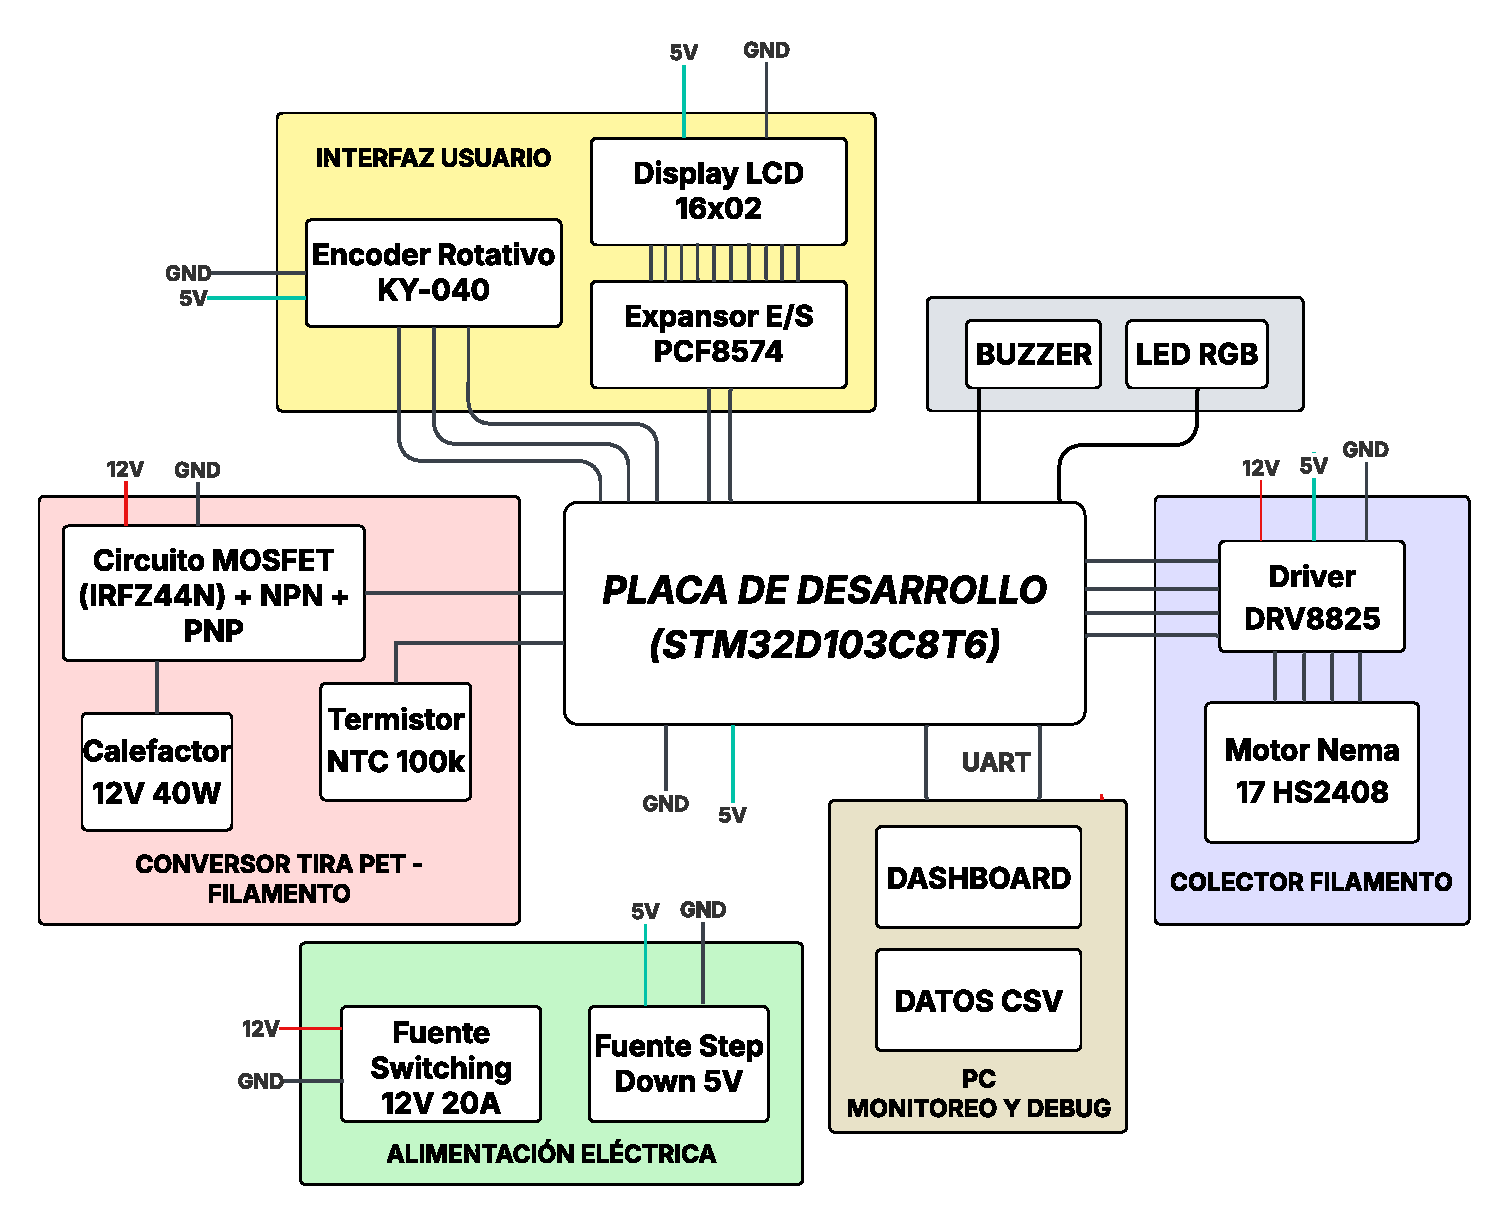
\includegraphics[width=\textwidth]{Mapa conceptual.pdf}
    \caption{Diagrama de bloques funcional de la extrusora de PET.}
    \label{fig:esquema}
\end{figure}

\section{Detalle de Módulos}
\textit{Nota: Los pines del microcontrolador mencionados en esta sección corresponden a la asignación configurada en STM32CubeMX. La configuración específica de cada periférico se detalla en la Sección 5 (Programación).}

\subsection{Microcontrolador: STM32F103 (Blue Pill)}
El núcleo del sistema es el microcontrolador \textbf{STM32F103C8T6}, basado en arquitectura ARM Cortex-M3 de 32 bits operando a 72 MHz.
\begin{itemize}
    \item \textbf{Conversión ADC con DMA}: Adquisición continua de la señal del termistor sin consumir ciclos de CPU.
    \item \textbf{Timers}: Generación de señales PWM para el calefactor y pulsos de paso para el motor.
    \item \textbf{Periféricos de comunicación}: I2C para el LCD, UART para telemetría PC y GPIO para botones/encoder.
    \item \textbf{Memoria Flash}: 64 KB, de los cuales se reserva una página (1 KB) para almacenamiento no volátil de parámetros PID y setpoints.
\end{itemize}

\subsection{Sistema de Alimentación y Regulación}
El sistema es alimentado por una fuente conmutada de \textbf{12V/20A}, suficiente para manejar las cargas combinadas del cartucho calefactor (40W) y el motor paso a paso. La distribución de potencia se realiza de la siguiente forma:
\begin{itemize}
    \item \textbf{Bus de 12V}: Alimenta directamente el cartucho calefactor (vía MOSFET), el driver DRV8825 y el regulador step-down.
    \item \textbf{Bus de 5V (LM2596)}: Regulador conmutado que alimenta la Bluepill, el LCD I2C, encoder rotativo, LED RGB y buzzer.
    \item \textbf{Bus de 3.3V}: Suministrado por el regulador interno del STM32 (AMS1117 de la placa Blue Pill) para la lógica digital.
\end{itemize}

\subsection{Control de Tracción: Motor Paso a Paso y Driver}
El avance del filamento se realiza mediante un motor paso a paso \textbf{NEMA 17 modelo 17HS2408} con las siguientes características:
\begin{itemize}
    \item Ángulo de paso: 1.8° (200 pasos/revolución)
    \item Corriente nominal: 0.6A por bobina
    \item Torque de retención: 0.4 Nm
\end{itemize}

El control del motor se efectúa mediante el driver \textbf{DRV8825}, configurado en modo de \textbf{1/32 micropasos}, resultando en 6400 pasos por revolución. Esta subdivisión garantiza un movimiento suave y reduce las vibraciones mecánicas que afectarían la uniformidad del filamento.

\textbf{Pines del STM32 utilizados:}
\begin{itemize}
    \item \texttt{PA8 (TIM1\_CH1)}: Señal STEP (pulsos de paso generados por Timer)
    \item \texttt{PA1}: Señal DIR (dirección de giro)
    \item \texttt{PA5}: Señal ENABLE (habilitación del driver)
    \item \texttt{PA11}: Señal FAULT (detección de fallos del driver)
\end{itemize}

\textbf{Relación de Transmisión}: El motor se acopla a un reductor de engranajes de relación de transmisión 60:1, multiplicando el torque disponible.

\textbf{Forma de manejo}: El control se realiza mediante tres señales digitales. La señal STEP es generada automáticamente por un Timer configurado en modo PWM, donde la frecuencia del tren de pulsos determina la velocidad de giro. La señal DIR (nivel alto/bajo) establece el sentido de rotación, y ENABLE activa o desactiva el driver. La señal FAULT permite detectar condiciones de error en el driver (sobrecalentamiento, cortocircuito).

\subsection{Control de Temperatura: Sensado y Actuación Térmica}
El sistema térmico consta de dos elementos integrados en un bloque calefactor de aluminio tipo \textbf{E3D V6}:

\subsubsection{Sensor de Temperatura (NTC 100k$\Omega$)}
\begin{itemize}
    \item Termistor negativo encapsulado en tubo metálico de 3mm de diámetro.
    \item Rango de operación: -50°C a 300°C.
    \item Conexión: Divisor resistivo con $R_{serie} = 1k\Omega$ conectado a \texttt{PA0 (ADC1\_CH0)}.
    \item El firmware aplica corrección mediante \textbf{ecuación Beta del termistor} con dos constantes Beta (3950 para baja temperatura, 4410 para alta temperatura) para compensar la no linealidad en el rango 200-250°C.
\end{itemize}

\begin{figure}[H]
    \centering
    %\includegraphics[width=0.6\textwidth]{circuito_ntc.png} % TODO: Agregar imagen del circuito NTC
    \caption{Circuito de acondicionamiento de señal para el termistor NTC.}
    \label{fig:circuito_ntc}
\end{figure}

\subsubsection{Actuador Térmico (Cartucho Calefactor)}
Para la gestión térmica se utiliza una resistencia de 12V/40W (aprox. $3.6\Omega$) controlada mediante una etapa de potencia.

Se diseñó un circuito basado en un transistor MOSFET de canal N \textbf{IRFZ44N}, configurado como interruptor de estado sólido. Esta etapa permite al microcontrolador, mediante una señal PWM de 3.3V en el pin \texttt{PB10}, conmutar la carga de 12V necesarios para el cartucho.

Debido a que el IRFZ44N no es un dispositivo de nivel lógico, se implementó un driver de gate de 12V (push-pull con transistores \textbf{BC327} y \textbf{BC337}) para asegurar la completa saturación del componente. Esto evita que el transistor trabaje en su zona lineal, lo que provocaría un sobrecalentamiento destructivo por $R_{DS(on)}$.

\begin{figure}[H]
    \centering
    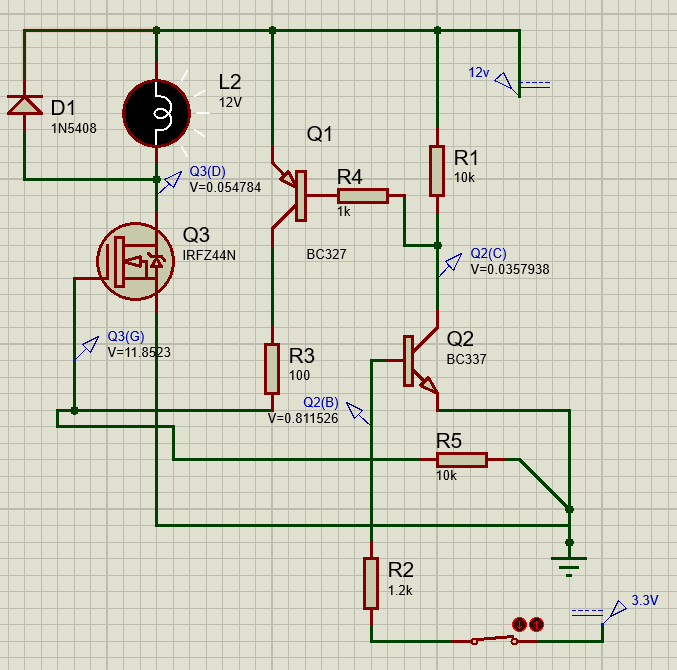
\includegraphics[width=0.6\textwidth]{circuito_heater.png} 
    \caption{Circuito de control de potencia mediante MOSFET para el cartucho calefactor.}
    \label{fig:circuito_potencia}
\end{figure}

\textbf{Forma de manejo}: La lectura del termistor se realiza mediante el conversor ADC en modo DMA, que captura 64 muestras de forma autónoma sin intervención del procesador. El firmware promedia estas muestras, calcula la resistencia del termistor mediante la ley de Ohm en el divisor resistivo, y aplica la \textbf{ecuación Beta} para obtener la temperatura en grados Celsius. El control del calefactor se efectúa mediante una señal digital ON/OFF en el pin PB10, que activa la etapa de driver la cual conmuta el MOSFET de potencia según la salida del controlador PID.

\subsection{Interfaz de Usuario Local}

\subsubsection{LCD 1602 I2C}
Para la visualización de parámetros y menús se utiliza un display alfanumérico de \textbf{16 columnas × 2 filas} con módulo adaptador I2C basado en el chip \textbf{PCF8574}. Este conversor reduce los 8 pines de datos paralelos del LCD a solo 2 líneas (SDA y SCL), simplificando el cableado.

\textbf{Características:}
\begin{itemize}
    \item Dirección I2C: \texttt{0x27} (7 bits) / \texttt{0x4E} (formato 8 bits de la HAL)
    \item Pines del STM32: \texttt{PB6 (I2C1\_SCL)} y \texttt{PB7 (I2C1\_SDA)}
    \end{itemize}

El LCD muestra en tiempo real: temperatura actual/objetivo, estado térmico (calentando/listo), velocidad del motor en Hz y mm/s, y mensajes de alarma en caso de fallo.

\textbf{Forma de manejo}: La comunicación con el LCD se realiza mediante el protocolo I2C utilizando las funciones de la biblioteca HAL. El PCF8574 actúa como expansor de puertos, recibiendo bytes de comando y datos que son traducidos a las señales paralelas que requiere el controlador HD44780 del LCD. 

\subsubsection{Encoder Rotativo con Pulsador}
La navegación por el menú de configuración se realiza mediante un \textbf{encoder rotativo incremental de 20 pulsos por revolución} con pulsador integrado.

\textbf{Conexión al STM32:}
\begin{itemize}
    \item \texttt{PB13}: Señal A (CLK)
    \item \texttt{PB14}: Señal B (DT)
    \item \texttt{PB15}: Pulsador (SW)
\end{itemize}

\textbf{Forma de manejo}: El encoder genera dos señales cuadradas desfasadas 90° (A y B). La lectura del sentido de giro se determina comparando el estado de la señal B cuando ocurre un flanco en A: si B está en alto, el giro es horario; si está en bajo, es antihorario. El pulsador se lee como un botón estándar con pull-up. El firmware mide el tiempo de pulsación para discriminar entre acción corta (confirmación) y larga (cambio de modo).

\subsection{Sistema de Señalización}

\subsubsection{LED RGB de Estado}
Se utiliza un LED RGB de cátodo común para indicar visualmente el estado operativo del sistema:

\textbf{Código de colores implementado:}
\begin{itemize}
    \item \textbf{Amarillo}: Sistema en reposo (Idle), listo para iniciar.
    \item \textbf{Azul}: Calentamiento inicial (T $<$ Target - 20°C).
    \item \textbf{Cyan}: Aproximación térmica (T $>$ Target - 20°C).
    \item \textbf{Verde}: Temperatura estable en rango $\pm5^\circ C$, listo para extruir.
    \item \textbf{Rojo parpadeante (500ms)}: Alarma de seguridad activa.
\end{itemize}

\textbf{Pines del STM32:}
\begin{itemize}
    \item \texttt{PA3}: Canal Rojo
    \item \texttt{PB0}: Canal Verde
    \item \texttt{PB1}: Canal Azul
\end{itemize}

\textbf{Forma de manejo}: Cada canal del LED se controla mediante una salida GPIO configurada en modo push-pull. Al ser un LED de cátodo común, se requiere nivel alto (3.3V) para encender cada color. Las combinaciones de colores se logran activando dos o tres canales simultáneamente.

\subsubsection{Buzzer Activo}
Zumbador piezoeléctrico de 5V para retroalimentación auditiva:
\begin{itemize}
    \item \textbf{Beeps cortos (50-100ms)}: Confirmación de pulsación de botón o cambio de parámetro.
    \item \textbf{Beeps intermitentes (500ms)}: Alarma de error crítico (desconexión de sensor, sobretemperatura, timeout de calentamiento). Sincronizado con el parpadeo del LED rojo.
    \item Pin de control: \texttt{PA2}
\end{itemize}

\textbf{Forma de manejo}: El buzzer se activa mediante una salida GPIO simple. Al ser un modelo activo, solo requiere alimentación (nivel alto) para generar el tono. El firmware controla la duración de los beeps mediante temporizadores no bloqueantes basados en \texttt{HAL\_GetTick()}.

\subsection{Botones de Control Físico}
El sistema incorpora tres pulsadores para el control directo del proceso:

\begin{itemize}
    \item \texttt{PA4 (START\_BTN)}: Inicia el motor de tracción (solo si la temperatura es segura $>100^\circ C$).
    \item \texttt{PB12 (STOP\_BTN)}: Detiene el motor.
    \item \texttt{PB11 (HEATER\_BTN)}: Conmuta el calentador entre ON/OFF (modo toggle).
\end{itemize}

Todos los botones implementan lógica pull-up interna y \textbf{filtrado temporal (200-300ms)} para evitar lecturas erróneas causadas por las vibraciones mecánicas que ocurren al presionar y soltar el contacto.

\textbf{Forma de manejo}: Los botones se leen mediante entradas GPIO configuradas con resistencias pull-up internas. El estado de reposo es nivel alto (3.3V), y al presionar se detecta nivel bajo (GND). Para evitar múltiples detecciones causadas por el rebote mecánico del contacto, el firmware ignora cualquier cambio de estado durante un período de 200-300ms después de la primera detección válida. Esto asegura que solo se registre una pulsación por cada acción real del usuario.

\subsection{Comunicación Serial UART}
El sistema integra un canal de comunicación bidireccional vía \textbf{UART} para supervisión remota y ajuste de parámetros desde PC.

\textbf{Configuración:}
\begin{itemize}
    \item Periférico: \texttt{USART1}
    \item Baudrate: 115200 bps, 8N1 (8 bits de datos, sin paridad, 1 bit de stop)
    \item Pines: \texttt{PA9 (TX)} y \texttt{PA10 (RX)}
\end{itemize}

\textbf{Protocolo implementado:}
\begin{itemize}
    \item \textbf{Telemetría (100ms)}: Envío continuo de datos en formato CSV: timestamp, temperatura actual, target, PWM, velocidad, error PID, código de error y flags de estado.
    \item \textbf{Comandos ASCII}: Recepción de instrucciones para cambio de setpoint (\texttt{T250}), encendido/apagado de calefactor (\texttt{H1/H0}), arranque/parada de motor (\texttt{R/S}), ajuste de PID (\texttt{P/I/D}), guardado en Flash (\texttt{W}) y reset a valores de fábrica (\texttt{X}).
\end{itemize}

La aplicación de PC (Python/Tkinter) visualiza gráficos en tiempo real, permite control remoto y registra automáticamente logs de telemetría y eventos de seguridad en archivos CSV.

% --- SECCIÓN 4: FUNCIONAMIENTO GENERAL ---
\section{Funcionamiento General}

\subsection{Arquitectura del Firmware}
El firmware implementa una arquitectura de \textbf{Superloop} (bucle principal infinito) con sincronización temporal precisa mediante interrupciones de Timer. Esta estrategia es común en sistemas embebidos de tiempo real, ya que permite respuestas deterministas sin la sobrecarga de un RTOS.

\subsubsection{Timers del Sistema}
El sistema utiliza dos periféricos timer con funciones específicas:

\textbf{TIM1 (Advanced Timer) - Generador PWM para Motor:}
\begin{itemize}
    \item Opera a 1 MHz (prescaler 72 desde 72 MHz de reloj del sistema).
    \item Genera la señal STEP en PA8 mediante PWM de frecuencia variable.
    \item El período (ARR) se ajusta dinámicamente según velocidad requerida: \texttt{ARR = (1000000 / freq\_hz) - 1}.
    \item Duty cycle fijo al 50\% para pulsos simétricos.
    \item Rango operativo: 50 Hz a 20 kHz.
\end{itemize}

\textbf{TIM3 (General Purpose Timer) - Base de Tiempo del Sistema:}
\begin{itemize}
    \item Configurado a 1 kHz (prescaler 7200, período 10), genera una interrupción cada 1 ms.
    \item Genera dos flags temporales no bloqueantes:
    \begin{itemize}
        \item \texttt{flag\_1ms}: Dispara actualización de rampa S del motor (cada ciclo).
        \item \texttt{flag\_100ms}: Dispara procesamiento ADC, PID térmico, telemetría UART y actualización LCD (contador interno: 100 ciclos).
    \end{itemize}
    \item Actúa como "reloj maestro" que sincroniza todas las tareas del sistema.
\end{itemize}

\subsubsection{Adquisición de Temperatura (ADC + DMA)}
El sensado térmico opera de forma completamente autónoma sin intervención del CPU:

\begin{itemize}
    \item \textbf{ADC1}: Configurado en modo continuo para lectura del canal 0 (PA0 - divisor resistivo con NTC 100k$\Omega$).
    \item \textbf{DMA1\_Channel1}: Transfiere automáticamente cada conversión ADC a un buffer de 64 muestras (\texttt{adc\_buffer[64]}).
    \item Cada 100 ms (flag\_100ms), el firmware:
    \begin{enumerate}
        \item Inicia nueva captura DMA de 64 conversiones.
        \item Calcula promedio aritmético del buffer para reducir ruido.
        \item Convierte el valor ADC promedio a temperatura mediante ecuación Beta.
        \item Aplica filtro IIR de primer orden ($\alpha = 0.1$) para suavizado adicional.
    \end{enumerate}
    \item Esta estrategia reduce significativamente el ruido eléctrico sin sobrecargar el procesador.
\end{itemize}

\subsubsection{Bucle Principal (Superloop)}
El \texttt{while(1)} ejecuta de forma iterativa las siguientes tareas:
\begin{enumerate}
    \item \textbf{Refrescar Watchdog (IWDG)}: Evita reset por timeout si el firmware se bloquea.
    \item \textbf{Lectura de entradas}: Encoder, botones físicos, comandos UART entrantes.
    \item \textbf{Gestión de alarmas}: Verificación continua del sistema de errores (prioridad máxima).
    \item \textbf{Ejecución condicional según flags temporales}:
    \begin{itemize}
        \item Si \texttt{flag\_1ms}: Llamada a \texttt{motor\_state\_machine()}.
        \item Si \texttt{flag\_100ms}: Procesamiento ADC, cálculo PID, envío de telemetría.
    \end{itemize}
    \item \textbf{Gestión de menú o actualización de pantalla}: Según el modo activo.
\end{enumerate}

\subsection{Máquina de Estados Térmica}
El control térmico está implementado como una FSM con 4 estados principales:

\textbf{Estados definidos:}
\begin{itemize}
    \item \textbf{THERMAL\_IDLE}: Sistema en reposo, calefactor OFF. Espera comando de inicio (botón físico o UART).
    \item \textbf{THERMAL\_HEATING}: Calefactor activo, algoritmo PID regulando potencia. 
    \begin{itemize}
        \item Se activa un temporizador de seguridad (5 minutos). Si no se alcanzan 100$^{\circ}$C en ese tiempo, se dispara \texttt{ERROR\_HEATING\_TIMEOUT}.
        \item LED: Azul (T $<$ Target-20$^{\circ}$C) o Cyan (T $>$ Target-20$^{\circ}$C).
    \end{itemize}
    \item \textbf{THERMAL\_READY}: Temperatura estabilizada ($|T_{actual} - T_{target}| < 5^{\circ}$C). PID sigue activo para compensar perturbaciones. LED Verde.
    \item \textbf{THERMAL\_ERROR}: Fallo de seguridad detectado. Calefactor cortado, motor detenido, alarma visual/sonora. \textbf{Requiere reconocimiento manual} (presionar START) para salir.
\end{itemize}

\textbf{Transiciones:}
\begin{itemize}
    \item IDLE $\rightarrow$ HEATING: Botón Heater o comando UART \texttt{H1}.
    \item HEATING $\rightarrow$ READY: $|Error| < 5^{\circ}$C.
    \item READY $\rightarrow$ HEATING: Temperatura sale del rango por carga térmica (extrusión).
    \item Cualquier estado $\rightarrow$ ERROR: Desconexión NTC, sobretemperatura ($T > 275^{\circ}$C), timeout de calentamiento.
    \item ERROR $\rightarrow$ IDLE: Solo mediante presión prolongada del botón START (reset intencional).
\end{itemize}

\subsection{Máquina de Estados del Motor}
La tracción mecánica también opera como FSM, con perfiles de aceleración suavizados mediante \textbf{curva S} (función coseno) para evitar sacudidas y vibraciones que afectarían la uniformidad del filamento.

\textbf{Estados definidos:}
\begin{itemize}
    \item \textbf{MOTOR\_IDLE}: Motor deshabilitado, frecuencia = 0 Hz.
    \item \textbf{MOTOR\_ACCEL}: Aceleración gradual desde frecuencia mínima (50 Hz) hasta frecuencia objetivo. Duración: 2000 pasos de rampa ($\sim$2 segundos a 1 kHz).
    \item \textbf{MOTOR\_RUN}: Velocidad constante. Si cambia el setpoint de velocidad, se ajusta gradualmente (5 Hz por ciclo).
    \item \textbf{MOTOR\_DECEL}: Deceleración suave hasta frecuencia mínima, seguida de apagado. Duración: 2000 pasos de rampa.
\end{itemize}

\textbf{Protección "Cold Protect":} El arranque del motor está bloqueado si $T_{actual} < 100^{\circ}$C, evitando obstrucciones mecánicas por filamento solidificado.

\textbf{Transiciones:}
\begin{itemize}
    \item IDLE $\rightarrow$ ACCEL: Botón START o comando UART \texttt{R}, solo si temperatura es segura.
    \item ACCEL $\rightarrow$ RUN: Completados 2000 pasos de rampa.
    \item RUN $\rightarrow$ DECEL: Botón STOP, comando UART \texttt{S}, o temperatura cae bajo umbral de seguridad.
    \item DECEL $\rightarrow$ IDLE: Completada rampa de frenado.
\end{itemize}

\subsection{Sistema de Seguridad Multicapa}

\subsubsection{Detección de Errores Críticos}
El firmware verifica continuamente las siguientes condiciones de fallo:

\begin{enumerate}
    \item \textbf{ERROR\_NTC\_DISCONNECTED}: Lectura ADC fuera de rango (< 100 o > 4000 cuentas digitales) o valor de temperatura = NaN (Not a Number). Indica cable suelto o sensor dañado.
    \item \textbf{ERROR\_OVERTEMP}: Temperatura excede 275$^{\circ}$C. Protección contra fuga térmica por fallo del PID o cortocircuito del MOSFET.
    \item \textbf{ERROR\_HEATING\_TIMEOUT}: No se alcanzaron 100$^{\circ}$C después de 5 minutos de calentamiento. Indica calefactor desconectado, contacto térmico deficiente o fallo en la etapa de potencia.
\end{enumerate}

\subsubsection{Enclavamiento de Seguridad (Safety Latch)}
A diferencia de alarmas simples que auto-resetean al desaparecer la causa, este sistema implementa \textbf{latch de error}: una vez disparada la alarma, el sistema permanece bloqueado incluso si la condición se corrige (ej: reconectar el sensor). El usuario \textbf{debe presionar manualmente el botón START} para reconocer el evento y volver a modo IDLE. Esta filosofía evita reinicios automáticos peligrosos en equipos de alta temperatura.

\subsubsection{Watchdog Independiente (IWDG)}
El perro guardián interno (Independent Watchdog) del STM32 está configurado para resetear el microcontrolador si no se refresca cada ~250 ms. Esto protege contra bloqueos del firmware por errores de software no previstos. El comando \texttt{HAL\_IWDG\_Refresh()} se ejecuta en cada iteración del loop principal.

\subsection{Interacción de Módulos y Flujo de Ejecución}
A continuación se describe el flujo típico de operación del sistema:

\textbf{Secuencia de arranque:}
\begin{enumerate}
    \item Usuario presiona botón HEATER (PB11) o envía \texttt{H1} por UART.
    \item Sistema transita a \texttt{THERMAL\_HEATING}, activa PID y comienza calentamiento.
    \item Cada 100 ms: ADC captura 64 muestras del termistor (DMA automático), firmware calcula temperatura mediante ecuación Beta y ejecuta PID. Salida PID determina si el pin PB10 está alto (calefactor ON) o bajo (OFF).
    \item LED RGB indica progreso: Azul (lejano del target) → Cyan (aproximándose) → Verde (listo).
    \item Al alcanzar temperatura, sistema transita a \texttt{THERMAL\_READY}.
\end{enumerate}

\textbf{Secuencia de extrusión:}
\begin{enumerate}
    \item Usuario presiona START (PA4). Firmware verifica temperatura segura ($>100^{\circ}$C).
    \item Si es seguro: motor transita a MOTOR\_ACCEL. Timer 1 genera pulsos STEP en PA8 con frecuencia creciente según curva S.
    \item Tras 2 segundos, motor alcanza velocidad objetivo (ej: 1500 Hz = 3 mm/s de filamento).
    \item Bucle PID térmico compensa la pérdida de calor por flujo de material.
    \item Al presionar STOP (PB12), motor decelera suavemente y se detiene.
\end{enumerate}

\textbf{Telemetría continua:}
\begin{itemize}
    \item Cada 100 ms, el firmware envía por UART un paquete CSV: \texttt{timestamp, T\_actual, T\_target, PWM\%, velocidad\_mm/s, error\_PID, codigo\_error, flags}.
    \item La aplicación Python recibe estos datos, grafica en tiempo real y registra logs en archivos CSV para análisis post-proceso.
\end{itemize}

\subsection{Diagrama de Flujo Operativo}
\begin{figure}[H]
    \centering
    \resizebox{\textwidth}{!}{
    \begin{tikzpicture}[node distance=0.7cm,
        startstop/.style={ellipse, draw, fill=green!20, text width=2cm, align=center, minimum height=0.9cm},
        process/.style={rectangle, draw, fill=blue!15, text width=3.2cm, align=center, minimum height=0.7cm, rounded corners},
        decision/.style={diamond, draw, fill=orange!20, text width=2.3cm, align=center, aspect=2},
        error/.style={rectangle, draw, fill=red!25, text width=2.3cm, align=center, minimum height=0.8cm},
        fsm/.style={rectangle, draw, fill=cyan!10, text width=2.3cm, align=center, minimum height=0.7cm, rounded corners},
        arrow/.style={-Stealth, thick},
        annotation/.style={text width=2cm, align=center, font=\small}]
        
        % Columna principal (centro)
        \node[startstop] (start) {INICIO};
        \node[process, below=of start] (init) {Inicializar periféricos \\ Cargar Config Flash \\ Arrancar TIM3, ADC \\ Estados $\rightarrow$ IDLE};
        \node[process, below=of init, fill=yellow!20, text width=2.5cm] (loop) {\textbf{WHILE}};
        \node[process, below=of loop] (wdg) {Refrescar Watchdog};
        \node[process, below=of wdg, fill=red!15] (alarm) {Gestionar Alarma/LED \\ (Error o Normal)};
        \node[process, below=of alarm] (inputs) {Leer botones \\ encoder, UART};
        \node[decision, below=of inputs, yshift=-0.4cm] (flag1ms) {¿flag\_1ms?};
        \node[decision, below=of flag1ms, yshift=-0.4cm] (flag100ms) {¿flag\_100ms?};
        \node[process, below=of flag100ms, yshift=-0.2cm] (lcd) {Actualizar LCD};
        
        % Columna derecha - Error crítico al costado
        \node[decision, right=4cm of inputs, yshift=-1cm] (error_check) {¿Error crítico?};
        \node[error, below=of error_check, yshift=-0.3cm] (error_mode) {MODO SEGURO \\ Apagar todo \\ Alarma};
        \node[decision, below=of error_mode, yshift=-0.2cm] (btn_reset) {¿Botón START?};
        \node[process, right=of btn_reset, xshift=0.5cm, fill=green!15] (clear_error) {Limpiar error \\ $\rightarrow$ IDLE};
        
        % Columna izquierda - Motor
        \node[fsm, left=2.8cm of flag1ms] (motor) {Actualizar Motor \\ (Rampa S)};
        \node[fsm, below=0.3cm of motor, fill=cyan!5, text width=2.3cm, minimum height=2.8cm] (motor_fsm) {
            \textbf{Motor FSM:} \\
            \small
            IDLE $\downarrow$ \\
            ACCEL (2s) $\downarrow$ \\
            RUN $\downarrow$ \\
            DECEL (2s) \\
            $\circlearrowleft$ IDLE
        };
        
        % Columna derecha - Temperatura
        \node[fsm, right=2.8cm of flag100ms] (thermal) {Procesar Temp \\ PID + Telemetría};
        \node[fsm, below=0.3cm of thermal, fill=orange!5, text width=2.3cm, minimum height=2.6cm] (thermal_fsm) {
            \textbf{Thermal FSM:} \\
            \small
            IDLE $\downarrow$ \\
            HEATING $\downarrow$ \\
            READY \\
            [2pt]
            $\rightarrow$ ERROR
        };
        
        % Flechas principales
        \draw[arrow] (start) -- (init);
        \draw[arrow] (init) -- (loop);
        \draw[arrow] (loop) -- (wdg);
        \draw[arrow] (wdg) -- (alarm);
        \draw[arrow] (alarm) -- (inputs);
        
        % Flecha de inputs a flag1ms CON PUNTO MEDIO para conectar a error_check
        \draw[arrow] (inputs) -- (flag1ms) coordinate[midway] (check1);
        \draw[arrow] (flag1ms) -- node[right, font=\footnotesize] {No} (flag100ms);
        \draw[arrow] (flag1ms) -- node[above, font=\footnotesize] {Sí} (motor);
        \draw[arrow] (motor) -- (flag1ms);
        
        % Flecha de flag100ms
        \draw[arrow] (flag100ms) -- node[right, font=\footnotesize] {No} (lcd);
        \draw[arrow] (flag100ms) -- node[above, font=\footnotesize] {Sí} (thermal);
        \draw[arrow] (thermal) -- (flag100ms) coordinate[midway] (check2);
        
        % Conexiones hacia error_check desde los puntos medios
        \draw[arrow, orange!70, thick] (check1) -- (error_check);
        \draw[arrow, orange!70, thick] (check2) -- (error_check);
        
        % Flujo de error
        \draw[arrow] (error_check) -- node[right, font=\footnotesize] {Sí} (error_mode);
        
        % Flujo de error y recuperación
        \draw[arrow] (error_mode) -- (btn_reset);
        \draw[arrow] (btn_reset) -- node[above, font=\footnotesize] {Sí} (clear_error);
        % Flecha roja que vuelve al WHILE: primero sube vertical, luego horizontal a la izquierda
        \draw[arrow, dashed, red] (clear_error.north) -- ++(0,8.5) |- (loop.north east);
        
        % Flecha de retorno al loop
        \draw[arrow, dashed] (lcd.west) -- ++(-1.2,0) |- (loop.west);
        
        % Anotaciones
        \node[annotation, left=0.2cm of motor_fsm, yshift=0.8cm, font=\scriptsize, text=blue!80] {TIM3 \\ cada 1ms};
        \node[annotation, right=0.2cm of thermal_fsm, yshift=0.8cm, font=\scriptsize, text=orange!80] {TIM3 \\ cada 100ms};
        
    \end{tikzpicture}
    }
    \caption{Diagrama de flujo del bucle principal y coordinación de máquinas de estado.}
    \label{fig:flujo}
\end{figure}

% --- SECCIÓN 5: PROGRAMACIÓN ---
\section{Programación}
\subsection{Configuración de Periféricos}
% Detalle de comunicación, A/D, PWM, sensores, drivers, etc.

\subsection{Descripción del Firmware}
% Descripción de main(), algoritmos, interrupciones, etc.

% --- SECCIÓN 6: ETAPAS DE MONTAJE Y ENSAYOS ---
\section{Etapas de Montaje y Ensayos Realizados}
% Describir pruebas parciales o conjuntas.

% --- SECCIÓN 7: RESULTADOS ---
\section{Resultados y Especificaciones Finales}
Explicitar el grado de cumplimiento de las metas y objetivos planteados inicialmente.
\begin{itemize}
    \item Consumo:
    \item Autonomía:
    \item Precisión:
    \item Velocidad:
    \item Rangos de trabajo:
\end{itemize}

% --- SECCIÓN 8: CONCLUSIONES ---
\section{Conclusiones}
Reflexión sobre el desarrollo realizado y perspectivas de mejoras del prototipo.
% Ejercicio de selección de componentes para producto comercial.

% --- REFERENCIAS ---
\section{Referencias}
\begin{enumerate}
    \item Hoja de datos STM32F103C8T6.
    \item Manual de referencia RM0008 STM32F101xx, STM32F102xx, STM32F103xx.
\end{enumerate}

% --- ANEXOS ---
\appendix
\section{Anexos}
% Detalles adicionales.

\end{document}